\chapter{Boundary and Interface Conditions}
\label{cha:boundary:interface:conditions}

\section{Assigning Boundary Conditions}

There are four basic steps in assigning a specific boundary condition
to a portion of the domain.
\begin{enumerate}
\item Create sets of vertices in the mesh generation process for each boundary
  condition.
\item Define boundary condition groups corresponding to the vertex sets.
\item Set the parameters for each boundary condition group using
  \filename{.cfg} files and/or command line
  arguments.
\item Specify the spatial variation in parameters for the boundary
  condition using a spatial database file.
\end{enumerate}

\subsection{Creating Sets of Vertices}

The procedure for creating sets of vertices differs depending on the
mesh generator. For meshes specified using the PyLith mesh ASCII
format, the sets of vertices are specified using groups (see Appendix
\vref{sec:format:MeshIOAscii}).  In CUBIT/Trelis the groups of
vertices are created using nodesets. Similarly, in LaGriT, psets are
used. Note that we chose to associate boundary conditions with groups
of vertices because nearly every mesh generation package supports
associating a string or integer with groups of vertices.  Note also
that we currently associate boundary conditions with string
identifiers, so even if the mesh generator uses integers, the name is
specified as the digits of the integer value. Finally, note that every
vertex set that ultimately is associated with a boundary condition on
a cell face (e.g., Neumann boundary conditions and fault interface
conditions) must correspond to a simply-connected surface.

\subsection{Arrays of Boundary Condition Components}

A dynamic array of boundary condition components associates a name
(string) with each boundary condition. This dynamic array of boundary
conditions replaces the boundary condition container in PyLith v1.0.
User-defined containers are no longer necessary, and the predefined
containers are no longer available (or necessary). The default boundary
condition for each component in the array is the \object{DirichletBC} object.
Other boundary conditions can be bound to the named items in the array
via a \filename{.cfg} file, \filename{.pml} file, or the command line.
The parameters for the boundary condition are set using the name of
the boundary condition. An example of setting the array of boundary
condition components and changing the types of boundary conditions
in a \texttt{.cfg} file:
\begin{cfg}
<h>[pylithapp.problem]</h>
<p>bc</p> = [x_neg, x_pos, y_pos, z_neg] ; Array of boundary conditions

# Default boundary condition is DirichletBC
# Keep default value for bc.x_neg
<f>bc.x_pos</f> = pylith.bc.DirichletBoundary ; change BC type to DirichletBoundary
<f>bc.y_pos</f> = pylith.bc.AbsorbingDampers ; change BC type to AbsorbingDampers
<f>bc.z_neg</f> = pylith.bc.Neumann ; change BC type to Neumann (traction)
\end{cfg}

\section{Time-Dependent Boundary Conditions}
\label{sec:boundary:conditions:time:dependent}

Several boundary conditions use a common formulation for the spatial
and temporal variation of the boundary condition parameters,
\begin{equation}
f(\vec{x})=f_{0}(\vec{x})+\dot{f}_{0}(\vec{x})(t-t_{0}(\vec{x}))+f_{1}(\vec{x})a(t-t_{1}(\vec{x})),
\end{equation}
where $f(\vec{x})$ may be a scalar or vector parameter, $f_{0}(\vec{x})$
is a constant value, $\dot{f}_{0}(\vec{x})$ is a constant rate of
change in the value, $t_{0}(\vec{x})$ is the onset time for the constant
rate of change, $f_{1}(\vec{x})$ is the amplitude for the temporal
modulation, $a(t)$ is the variation in amplitude with time, $t_{1}(\vec{x})$
is the onset time for the temporal modulation, and $\vec{x}$ is the
position of a location in space. This common formulation permits easy
specification of a scalar or vector with a constant value, constant
rate of change of a value, and/or modulation of a value in time. One
can specify just the initial value, just the rate of change of the
value (along with the corresponding onset time), or just the modulation
in amplitude (along with the corresponding temporal variation and
onset time), or any combination of the three. The facilities associated
with this formulation are:
\begin{inventory}
\facilityitem{db\_initial}{Spatial database specifying the spatial variation
in the initial value (default is none).}
\facilityitem{db\_rate}{Spatial database specifying rate of change in the value
(default is none).}
\facilityitem{db\_change}{Spatial database specifying the amplitude of the temporal
modulation (default is none).}
\facilityitem{th\_change}{Time history database specifying the temporal change
in amplitude (default is none).}
\end{inventory}

\subsection{Dirichlet Boundary Conditions}

Dirichlet boundary conditions in PyLith prescribe the displacement
of a subset of the vertices of the finite-element mesh. While Dirichlet
boundary conditions can be applied to any vertex, usually they are
applied to vertices on the lateral and bottom boundaries of the domain.
There are two types of Dirichlet boundary conditions, \object{DirichletBC}
and \object{DirichletBoundary}. Both provide identical constraints on the solution,
but \object{DirichletBoundary} is limited to vertices of a simply-connected
surface, which allows diagnostic output of the prescribed displacements.
\object{DirichletBC} can be applied to a set of unconnected vertices.

The properties and components common to both the \object{DirichletBC} and
\object{DirichletBoundary} boundary conditions are:
\begin{inventory}
\propertyitem{label}{Label of the group of vertices associated with the boundary
condition.}
\propertyitem{bc\_dof}{Array of degrees of freedom to be fixed (first degree
of freedom is 0).}
\end{inventory}
\object{DirichletBoundary} contains an additional component:
\begin{inventory}
\facilityitem{output}{Manager for output of displacements on boundary with specified
displacements.}
\end{inventory}
By default the output manager does not output any information. The
specified displacements and velocities can be output by including
``displacement'' and ``velocity'' in the output manager's \property{vertex\_info\_fields}
array parameter. An example of setting the Dirichlet boundary condition
parameters in a \filename{.cfg} file is:
\begin{cfg}
<h>[pylithapp.problem]</h>
<p>bc</p> = [mybc]

<h>[pylithapp.problem.bc.mybc]</h>
<p>label</p> = group A 
<p>bc_dof</p> = [2] ; fixed displacement in z direction
<f>db_initial</f> = spatialdata.spatialdb.SimpleDB
<p>db_initial.iohandler.filename</p> = disp_A.spatialdb
<p>db_initial.query_type</p> = nearest ; change query type to nearest point algorithm
<f>db_rate</f> = spatialdata.spatialdb.UniformDB
<p>db_rate.values</p> = [displacement-rate-z]
<p>db_rate.data</p> = [1.0e-06*m/s] ; velocity is 1.0e-06 m/s
\end{cfg}
We have created an array with one boundary condition, mybc. The group
of vertices associated with the boundary condition is group A. For the
database associated with the constant displacement, we use a
\object{SimpleDB}.  We set the filename and query type for the
database. For the rate of change of values, we use a UniformDB and
specify the velocity in the z-direction to be 1.0e-06 m/s. See Section
\vref{sec:spatial:databases} for a discussion of the different types
of spatial databases available.

\begin{table}[htbp]
  \caption{Fields available in output of \object{DirichletBoundary} boundary condition information.}
  \label{tab:dirichlet:output}
  \begin{tabular}{llp{3in}}
    \textbf{Field Type} & \textbf{Field} & \textbf{Description} \\
    \hline 
    \property{vertex\_info\_fields} & \texttt{displacement\_initial} & Initial displacement field in global coordinate system\\
    & \texttt{velocity} & Rate of change of displacement field in global coordinate system\\
    & \texttt{velocity\_start\_time} & Onset time in seconds for rate of change in displacement field\\
    & \texttt{displacement\_change} & Amplitude of change in displacement field in global coordinate system\\
    & \texttt{change\_start\_time} & Onset time in seconds for the amplitude change in the displacement field\\
    \hline 
  \end{tabular}
\end{table}

\subsubsection{Dirichlet Boundary Condition Spatial Database Files}

The spatial database files for the Dirichlet boundary condition specify
the fixed displacements. The spatial database file may contain displacements
at more degrees of freedom than those specified in the Dirichlet boundary
condition settings using the \property{bc\_dof} setting. Only those
listed in \property{bc\_dof} will be used. This permits using the same
spatial database file for multiple Dirichlet boundary conditions with
the same displacement field.

\begin{table}[htbp]
  \caption{Values in the spatial databases used for Dirichlet boundary conditions.}
  \begin{tabular}{lp{4in}}
    \textbf{Spatial database} & \textbf{Name in Spatial Database}\\
    \facility{db\_initial} & \texttt{displacement-x, displacement-y, displacement-z}\\
    \facility{db\_rate} & \texttt{displacement-rate-x, displacement-rate-y, displacement-rate-z, rate-start-time}\\
    \facility{db\_change} & \texttt{displacement-x, displacement-y, displacement-z, change-start-time}\\
    \hline 
  \end{tabular}
\end{table}


\subsection{Neumann Boundary Conditions}

Neumann boundary conditions are surface tractions applied over a subset
of the mesh. As with the DirichletBoundary condition, each Neumann
boundary condition can only be applied to a simply-connected surface.
The surface over which the tractions are applied always has a spatial
dimension that is one less than the dimension of the finite-element
mesh. Traction values are computed at the integration points of each
cell on the surface, using values from a spatial database. The tractions
are integrated over each cell and assembled to obtain the forces applied
at the vertices. See Section \vref{sec:examples:twoquad4-traction}
for a tutorial that uses Neumann boundary conditions.

\important{In the small (finite) strain formulation, we assume that
  the normal and shear tractions are prescribed in terms of the
  undeformed configuration as described in section
  \vref{sec:small:strain:formulation}.}

The Neumann boundary condition properties and components are:
\begin{inventory}
\propertyitem{label}{Name of the group of vertices defining the mesh boundary
for the Neumann boundary condition.}
\propertyitem{up\_dir}{This is a 3-vector that provides a hint for the direction
perpendicular to the horizontal tangent direction that is not collinear
with the direction normal to the surface. The default value is (0,0,1),
which assumes that the z-axis is positive upward. This vector is only
needed for three-dimensional problems where the positive upward direction
differs from the default.}
\facilityitem{output}{The output manager associated with diagnostic output (traction
vector).}
\facilityitem{quadrature}{The quadrature object to be used for numerical integration.
Since we are integrating over a surface that is one dimension lower
than the problem domain, this would typically be set to something
like \texttt{Quadrature2Din3D} (for a three-dimensional problem).}
\end{inventory}
By default the output manager does not output any information. The
specified tractions can be output in global coordinates by including
``tractions'' in the output manager's \property{cell\_info\_fields}
array parameter. An example of setting these parameters in a
\filename{.cfg} file is:
\begin{cfg}
<h>pylithapp.timedependent]</h>
<p>bc</p> = [x_neg, x_pos, y_neg]
<f>bc.x_pos</f> = pylith.bc.Neumann ; Change BC type to Neumann

<h>[pylithapp.timedependent.bc.x_pos]</h>
<p>label</p> = x_pos ; Name of group of vertices for +x boundary
<f>db_initial</f> = spatialdata.spatialdb.SimpleDB
<p>db_initial.label</p> = Neumann BC +x edge
<p>db_initial.iohandler.filename</p> = axialtract.spatialdb
<p>db_initial.query_type</p> = nearest
<f>quadrature.cell</f> = pylith.feassemble.FIATLagrange
<p>quadrature.cell.dimension</p> = 1
<p>quadrature.cell.quad_order</p> = 2
\end{cfg}
These settings correspond to the example problem described in Section
\vref{sec:examples:twoquad4-traction}. It is necessary to set the
boundary condition type to \object{pylith.bc.Neumann}, since the default
value is \object{DirichletBC}. Constant tractions are used for this
particular problem, so a quadrature order of one would have been sufficient;
however, for problems involving more complex variations (e.g., a linear
variation), a quadrature order of two will provide more accurate results.
Note that there is no advantage to specifying an integration order
higher than two, since linear elements are being used for this problem.

\begin{table}[htbp]
  \caption{Fields available in output of \object{Neumann} boundary condition information.}
  \label{tab:neumann:output}
  \begin{tabular}{llp{3in}}
    \textbf{Field Type} & \textbf{Field} & \textbf{Description}\\
    \hline 
    \property{cell\_info\_fields} & \texttt{tracton\_initial} & Initial traction field in global coordinate system\\
    & \texttt{traction\_rate} & Rate of change of traction field in global coordinate system\\
    & \texttt{rate\_start\_time} & Onset time in seconds for rate of change in traction field\\
    & \texttt{traction\_change} & Amplitude of change in traction field in global coordinate system\\
    & \texttt{change\_start\_time} & Onset time in seconds for the amplitude change in the traction field\\
    \hline 
  \end{tabular}
\end{table}


\subsubsection{Neumann Boundary Condition Spatial Database Files}

The spatial database files for the Neumann boundary condition specify
the applied tractions. The number of traction components is equal
to the spatial dimension for the problem. The tractions are specified
in a local coordinate system for the boundary. The names of the components
of the traction vector are:
\begin{description}
\item [one-dimensional] \texttt{normal}
\item [two-dimensional] \texttt{shear}, \texttt{normal}
\item [three-dimensional] \texttt{horiz-shear}, \texttt{vert-shear}, \texttt{normal}
\end{description}
Ambiguities in specifying the shear tractions in 3D problems are resolved
using the \property{up\_dir} parameter. In the case of a horizontal
surface, users will need to pick an alternative vector, as the default
\property{up\_dir} would coincide with the normal direction. In this
case, the orientation for the \texttt{vert-shear-traction} component
will correspond to whatever the user specifies for \property{up\_dir},
rather than the actual vertical direction.

\begin{table}[htbp]
  \caption{Values in the spatial databases used for Dirichlet boundary conditions
    in three dimensions. In one- and two-dimensional problems, the names
    of the components are slightly different as described earlier in this
    section.}
  \begin{tabular}{lp{4in}}
    \textbf{Spatial database} & \textbf{Name in Spatial Database}\\
    \hline 
    \facility{db\_initial} & \texttt{traction-shear-horiz, traction-shear-vert, traction-normal}\\
    \facility{db\_rate} & \texttt{traction-rate-horiz-shear, traction-rate-vert-shear, traction-rate-normal,rate-start-time}\\
    \facility{db\_change} & \texttt{traction-horiz-shear, traction-vert-shear, traction-normal,change-start-time}\\
    \hline 
  \end{tabular}
\end{table}


\subsection{Point Force Boundary Conditions}

Point force boundary conditions in PyLith prescribe the application
of point forces to a subset of the vertices of the finite-element
mesh. While point force boundary conditions can be applied to any
vertex, usually they are applied to vertices on the lateral, top,
and bottom boundaries of the domain.

\subsubsection{Point Force Parameters}

The properties and components for the \object{PointForce} boundary
condition are:
\begin{inventory}
\propertyitem{label}{Label of the group of vertices associated with the boundary condition.}
\propertyitem{bc\_dof}{Array of degrees of freedom to which forces are applied (first degree of freedom is 0).}
\end{inventory}
An example of setting the point force boundary condition parameters
in a \filename{.cfg} file is:
\begin{cfg}
<h>[pylithapp.problem]</h>
<p>bc</p> = [mybc]
<f>bc.mybc</f> = pylith.bc.PointForce

<h<[pylithapp.problem.bc.mybc]</h>
<p>label</p> = group A 
<p>bc_dof</p> = [2] ; force in z direction
<f>db_initial</f> = spatialdata.spatialdb.SimpleDB
<p>db_initial.iohandler.filename</p> = force\_A.spatialdb
<p>db_initial.query_type</p> = nearest ; change query type to nearest point algorithm
<f>db_rate</f> = spatialdata.spatialdb.UniformDB
<p>db_rate.values</p> = [force-rate-z]
<p>db_rate.data</p> = [1.0e+5*newton/s]
\end{cfg}
We have created an array with one boundary condition, mybc. The group
of vertices associated with the boundary condition is group A. For
the database associated with the constant force, we use a SimpleDB.
We set the filename and query type for the database. For the rate
of change of values, we use a \object{UniformDB} and specify the rate of change
in the force to be 1.0e+5 Newton/s. See Section \vref{sec:spatial:databases}
for a discussion of the different types of spatial databases available.

\subsubsection{Point Force Spatial Database Files}

The spatial database files for the point force boundary condition specify
the forces applied. 

\begin{table}[htbp]
  \caption{Values in the spatial databases used for point force boundary conditions.}
  \begin{tabular}{lp{4in}}
    \textbf{Spatial database} & \textbf{Name in Spatial Database}\\
    \hline 
    \facility{db\_initial} & \texttt{force-x, force-y, force-z}\\
    \facility{db\_rate} & \texttt{force-rate-x, force-rate-y, force-rate-z, rate-start-time}\\
    \facility{db\_change} & \texttt{force-x, force-y, force-z, change-start-time}\\
    \hline 
  \end{tabular}
\end{table}


\section{Absorbing Boundary Conditions}
\label{sec:absorbing:boundaries}

This \object{AbsorbingDampers} boundary condition attempts to prevent seismic waves reflecting
off of a boundary by placing simple dashpots on the boundary. Normally
incident dilatational and shear waves are perfectly absorbed. Waves
incident at other angles are only partially absorbed. This boundary
condition is simpler than a perfectly matched layer (PML) boundary
condition but does not perform quite as well, especially for surface
waves. If the waves arriving at the absorbing boundary are relatively
small in amplitude compared to the amplitudes of primary interest,
this boundary condition gives reasonable results.

The \object{AbsorbingDampers} boundary condition properties and components are:
\begin{inventory}
\propertyitem{label}{Name of the group of vertices defining the mesh boundary
for the absorbing boundary condition.}
\propertyitem{up\_dir}{This is a 3-vector that provides a hint for the direction
perpendicular to the horizontal tangent direction that is not collinear
with the direction normal to the surface. The default value is (0,0,1),
which assumes that the z-axis is positive upward. This vector is only
needed for three-dimensional problems where the positive upward direction
differs from the default.}
\facilityitem{db}{The spatial database specifying the material properties for
the seismic velocities.}
\facilityitem{quadrature}{The quadrature object to be used for numerical integration.
Since we are integrating over a surface that is one dimension lower
than the problem domain, this would typically be set to something
like \facility{Quadrature2Din3D} (for a three-dimensional problem).}
\end{inventory}

\subsection{Finite-Element Implementation of Absorbing Boundary}

Consider a plane wave propagating at a velocity $c$. We can write
the displacement field as
\begin{equation}
\vec{u}(\vec{x},t)=\vec{u^{t}}(t-\frac{\vec{x}}{c}),
\end{equation}
where $\vec{x}$ is position, $t$ is time, and $\vec{u^{t}}$ is
the shape of the propagating wave. For an absorbing boundary we want
the traction on the boundary to be equal to the traction associated
with the wave propagating out of the domain. Starting with the expression
for the traction on a boundary, $T_{i}=\sigma_{ij}n_{j},$ and using
the local coordinate system for the boundary $s_{h}s_{v}n,$ where
$\vec{n}$ is the direction normal to the boundary, $\overrightarrow{s}_{h}$
is the horizontal direction tangent to the boundary, and $\overrightarrow{s}_{v}$
is the vertical direction tangent to the boundary, the tractions on
the boundary are
\begin{gather}
T_{s_{h}}=\sigma_{s_{h}n}\\
T_{s_{v}}=\sigma_{s_{v}n}\\
T_{n}=\sigma_{nn}.
\end{gather}
In the case of a horizontal boundary, we can define an auxiliary direction
in order to assign unique tangential directions. For a linear elastic
isotropic material, $\sigma_{ij}=\lambda\epsilon_{kk}\delta_{ij}+2\mu\epsilon_{ij},$
and we can write the tractions as 
\begin{gather}
T_{s_{h}}=2\mu\epsilon_{s_{h}n}\\
T_{s_{v}}=2\epsilon_{s_{v}n}\\
T_{n}=(\lambda+2\mu)\epsilon_{nn}+\lambda(\epsilon_{s_{h}s_{h}}+\epsilon_{s_{v}s_{v}}).
\end{gather}
For infinitesimal strains, $\epsilon_{ij}=\frac{1}{2}(u_{i,j}+u_{j,i})$
and we have
\begin{gather}
\epsilon_{s_{h}n}=\frac{1}{2}(u_{s_{h},n}+u_{n,s_{h}})\\
\epsilon_{s_{v}n}=\frac{1}{2}(u_{s_{v},n}+u_{n,s_{v}})\\
\epsilon_{nn}=u_{n,n}.
\end{gather}
For our propagating plane wave, we recognize that
\begin{equation}
\frac{\partial\vec{u^{t}}(t-\frac{\vec{x}}{c})}{\partial x_{i}}=-\frac{1}{c}\frac{\partial\vec{u^{t}}(t-\frac{\vec{x}}{c})}{\partial t},
\end{equation}
so that our expressions for the tractions become
\begin{gather}
T_{s_{h}}=-\frac{\mu}{c}\left(\frac{\partial u_{s_{h}}^{t}(t-\frac{\vec{x}}{c})}{\partial t}+\frac{\partial u_{n}^{t}(t-\frac{\vec{x}}{c})}{\partial t}\right),\\
T_{s_{v}}=-\frac{\mu}{c}\left(\frac{\partial u_{s_{v}}^{t}(t-\frac{\vec{x}}{c})}{\partial t}+\frac{\partial u_{n}^{t}(t-\frac{\vec{x}}{c})}{\partial t}\right).
\end{gather}
For the normal traction, consider a dilatational wave propagating
normal to the boundary at speed $v_{p}$; in this case $u_{s_{h}}=u_{s_{v}}=0$
and $c=v_{p}$. For the shear tractions, consider a shear wave propagating
normal to the boundary at speed $v_{s}$; we can decompose this into
one case where $u_{n}=u_{s_{v}}=0$ and another case where $u_{n}=u_{s_{h}}=0$,
with $c=v_{s}$ in both cases. We also recognize that $\mu=\rho v_{s}^{2}$
and $\lambda+2\mu=\rho v_{p}^{2}$. This leads to the following expressions
for the tractions:
\begin{gather}
T_{s_{h}}=-\rho v_{s}\frac{\partial u_{s_{h}}^{t}(t-\frac{\vec{x}}{c})}{\partial t}\\
T_{s_{v}}=-\rho v_{s}\frac{\partial u_{v}^{t}(t-\frac{\vec{x}}{c})}{\partial t}\\
T_{n}=-\rho v_{p}\frac{\partial u_{n}^{t}(t-\frac{\vec{x}}{c})}{\partial t}
\end{gather}
We write the weak form of the boundary condition as
\[
\int_{S_{T}}T_{i}\phi_{i}\, dS=\int_{S_{T}}-\rho c_{i}\frac{\partial u_{i}}{\partial t}\phi_{i}\, dS,
\]
where $c_{i}$ equals $v_{p}$ for the normal traction and $v_{s}$
for the shear tractions, and $\phi_{i}$ is our weighting function.
We express the trial solution and weighting function as linear combinations
of basis functions,
\begin{gather}
u_{i}=\sum_{m}a_{i}^{m}N^{m},\\
\phi_{i}=\sum_{n}c_{i}^{n}N^{n}.
\end{gather}
Substituting into our integral over the absorbing boundaries yields
\begin{equation}
\int_{S_{T}}T_{i}\phi_{i}\, dS=\int_{S_{T}}-\rho c_{i}\sum_{m}\dot{a}_{i}^{m}N^{m}\sum_{n}c_{i}^{n}N^{n}\, dS.
\end{equation}
In the derivation of the governing equations, we recognized that the
weighting function is arbitrary, so we form the residual by setting
the terms associated with the coefficients $c_{i}^{n}$ to zero,

\begin{equation}
r_{i}^{n}=\sum_{\text{tract cells}}\sum_{\text{quad pts}}-\rho(x_{q})c_{i}(x_{q})\sum_{m}\dot{a}_{i}^{m}N^{m}(x_{q})N^{n}(x_{q})w_{q}|J_{cell}(x_{q})|,
\end{equation}
 where $x_{q}$ are the coordinates of the quadrature points, $w_{q}$
are the weights of the quadrature points, and $|J_{cell}(x_{q})|$
is the determinant of the Jacobian matrix evaluated at the quadrature
points associated with mapping the reference cell to the actual cell.

The appearance of velocity in the expression for the residual means
that the absorbing dampers also contribute to the system Jacobian
matrix. Using the central difference method, the velocity is written
in terms of the displacements,
\begin{equation}
\dot{u}_{i}(t)=\frac{1}{2\Delta t}(u_{i}(t+\Delta t)-u_{i}(t-\Delta t)).
\end{equation}
Expressing the displacement at time $t+\Delta t$ in terms of the
displacement at time $t$ ($u_{i}(t)$) and the increment in the displacement
at time $t$ ($du_{i}(t)$) leads to
\begin{equation}
\dot{u}_{i}(t)=\frac{1}{2\Delta t}(du_{i}(t)+u_{i}(t)-u_{i}(t-\Delta t))
\end{equation}
The terms contributing to the system Jacobian are associated with
the increment in the displacement at time $t$. Substituting into
the governing equations and isolating the term associated with the
increment in the displacement at time t yields
\begin{equation}
A_{ij}^{nm}=\sum_{\text{tract cells}}\sum_{\text{quad pts}}\delta_{ij}\frac{1}{2\Delta t}\rho(x_{q})v_{i}(x_{q})N^{m}(x_{q})N^{n}(x_{q})w_{q}|J_{cells}(x_{q})|,
\end{equation}
where $A_{ij}^{mn}$ is an $nd$ by $md$ matrix ($d$ is the dimension
of the vector space), $m$ and $n$ refer to the basis functions and
$i$ and $j$ are vector space components.


\section{Fault Interface Conditions}
\label{sec:fault}

Fault interfaces are used to create dislocations (jumps in the displacement
field) in the model. The dislocations arise from slip across a fault
surface. Both shear and tensile dislocations are supported. For fault
interfaces, dislocations in 1D correspond to fault-opening (and closing),
in 2D lateral-slip and fault opening, and in 3D lateral-slip, reverse-slip,
and fault opening. PyLith supports kinematic (prescribed) slip and
dynamic (spontaneous) rupture simulations.

\subsection{Conventions}

Slip corresponds to relative motion across a fault surface. Figure
\vref{fig:fault:orientation} shows the orientation of the slip vector
in 3D with respect to the fault surface and coordinate axes. PyLith
automatically determines the orientation of the fault surface. This
alleviates the user from having to compute the strike, dip, and rake
angles over potentially complex, nonplanar fault surfaces. Instead,
the user specifies fault parameters in terms of lateral motion, reverse
motion, and fault opening as shown in Figure \vref{fig:fault:slip:motions}.

\begin{figure}[htbp]
  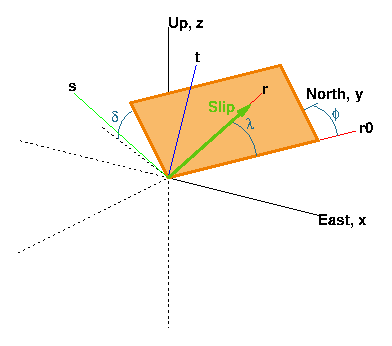
\includegraphics{boundaryconditions/figs/faultOrientation}
  \caption{Orientation of a fault surface in 3D, where $\phi$ denotes the angle
    of the fault strike, $\delta$ denotes the angle of the fault dip,
    and $\lambda$ the rake angle.}
  \label{fig:fault:orientation} 
\end{figure}

\begin{figure}[htbp]
  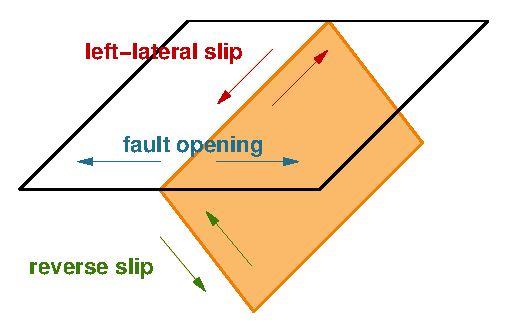
\includegraphics{boundaryconditions/figs/slipmotions}
  \caption{Sign conventions associated with fault slip. Positive values are associated
    with left-lateral, reverse, and fault opening motions.}
  \label{fig:fault:slip:motions} 
\end{figure}

\subsection{Fault Implementation}

In order to create relative motion across the fault surface in the
finite-element mesh, additional degrees of freedom are added along
with adjustment of the topology of the mesh. These additional degrees
of freedom are associated with cohesive cells. These zero-volume cells
allow control of the relative motion between vertices on the two sides
of the fault. PyLith automatically adds cohesive cells for each fault
surface. Figure \vref{fig:fault:cohesive:cells} illustrates the results
of inserting cohesive cells in a mesh consisting of triangular cells.
This example also shows the distinction between how buried fault edges
are handled differently than fault edges that reach the edge of the
domain, such as the ground surface.

\begin{figure}[htbp]
  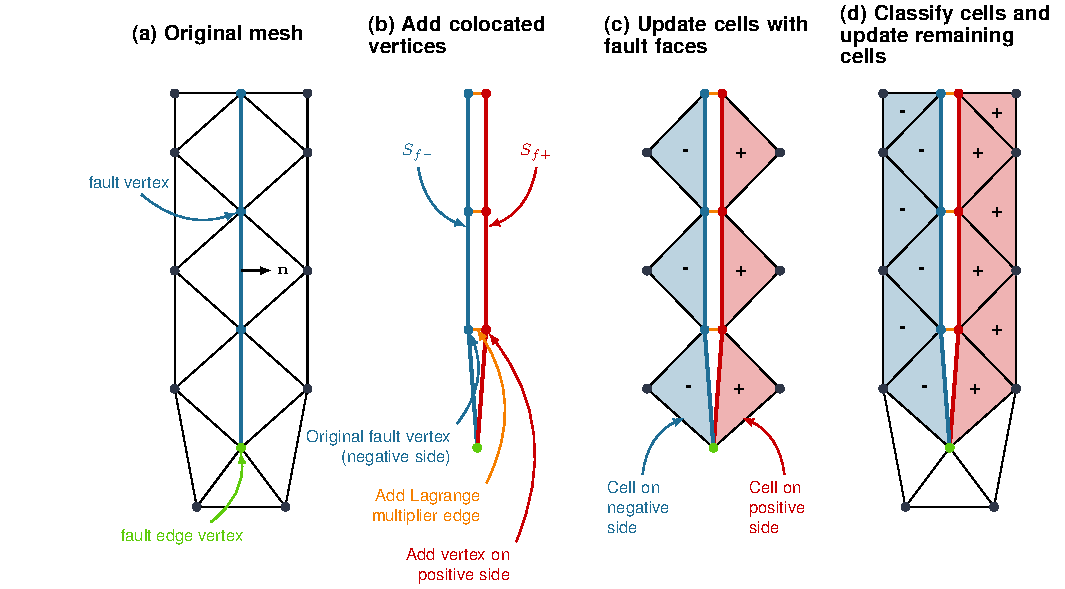
\includegraphics[width=6.25in]{boundaryconditions/figs/cohesivecell}
  \caption{Example of cohesive cells inserted into a mesh of
    triangular cells.  The zero thickness cohesive cells control slip
    on the fault via the relative motion between the vertices on the
    positive and negative sides of the fault.}
  \label{fig:fault:cohesive:cells} 
\end{figure}

\begin{figure}[htbp]
  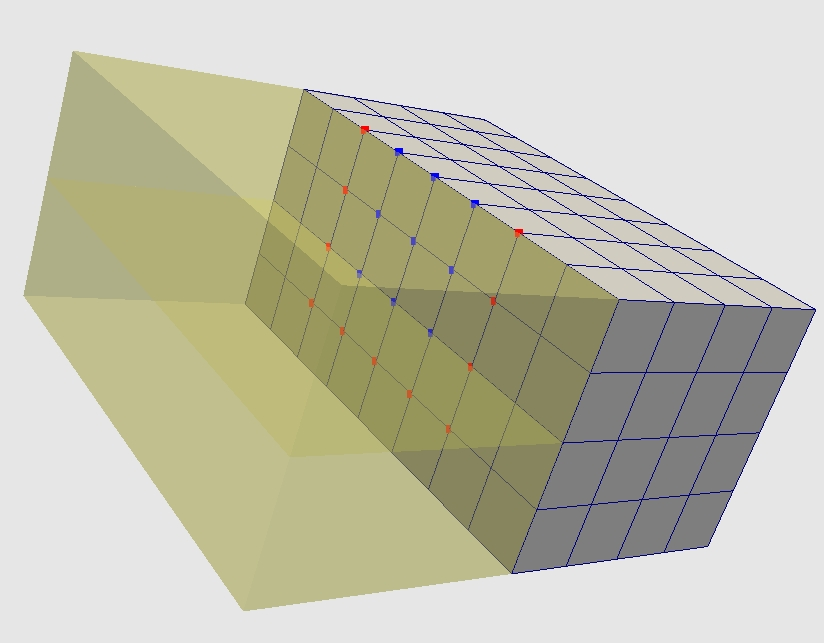
\includegraphics[width=4in]{boundaryconditions/figs/faultEdge}
  \caption{Example of how faults with buried edges must be described
    with two sets of vertices. All of the vertices on the fault are
    included in the \texttt{fault} group; the subset of vertices along
    the buried edges are included in the \texttt{fault\_edge}
    group. In 2-D the fault edges are just a single vertex as shown in
    Figure
    \vref{fig:fault:cohesive:cells}(a).}
  \label{fig:fault:fault_edge}
\end{figure}
For faults that have buried edges, splitting the mesh apart and inserting
the cohesive cells becomes complex at the buried edges due to the
ambiguity of defining where the fault ends and how to insert the cohesive
cell. In PyLith v2.0.0 we have changed how the buried edges of the
fault are managed. An additional group of fault nodes is specified
(e.g., via a nodeset from CUBIT) that marks the buried edges of the
fault (see Figure \vref{fig:fault:fault_edge}). This allows the cohesive
cell insertion algorithm to adjust the topology so that cohseive cells
are inserted up to the buried edge of the fault but no additional
degrees of freedom are added on the fault edge. This naturally forces
slip to zero along the buried edges.

\subsection{Fault Parameters}

The principal parameters for fault interface conditions are:
\begin{inventory}
\propertyitem{id}{This is an integer identifier for the fault surface. It is
used to specify the \property{material-id} of the cohesive cells in
the mesh. Material identifiers must be unique so this value cannot
be the same as any of the material models or any other fault.}
\propertyitem{label}{Name of group of vertices associated with the fault surface.
This label is also used in error and diagnostic reports.}
\propertyitem{edge}{Name of group of vertices marking the buried edges of the
fault.}
\propertyitem{up\_dir}{Up-dir or up direction (used in 2D and 3D simulations).
In 2D the default in-plane slip is left-lateral, so we use the up-direction
to resolve the ambiguity in specifying reverse slip. In 3D the up-direction
is used to resolve the ambiguity in the along-strike and dip-dir directions.
If the fault plane is horizontal, then the up-dir corresponds to the
reverse-motion on the +z side of the fault. The only requirement for
this direction is that it not be collinear with the fault normal direction.
The default value of [0, 0, 1] is appropriate for most 3D problems.}
\facilityitem{quadrature}{Quadrature object used in integrating fault quantities.}
\facilityitem{output}{Manager for output of diagnostic and data fields for the fault.}
\end{inventory}
By default the output manager outputs both diagnostic information
(e.g., fault normal direction) and the slip at each time step. Tables
\vref{tab:fault:kin:output} and \vref{tab:fault:dyn:output} list the
fields available for output for a fault with kinematic (prescribed)
earthquake rupture and a fault with dynamic rupture, respectively.
The fault coordinate system is shown in Figure \vref{fig:fault:slip:motions}.
The vectors in the fault coordinate system can be transformed to the
global coordinate system using the direction vectors in the diagnostic
output. An example of setting these parameters in a \filename{.cfg}
file is:
\begin{cfg}
<h?[pylithapp.problem]</h>
<p>interfaces</p> = [fault] 

<h>[pylithapp.problem.interfaces]</h>
<f>fault</f> = pylith.faults.FaultCohesiveKin ; default
<p>label</p> = fault_A ; Group of vertices defining the fault surface
<p>edge</p> = fault_edge ; Group of vertices defining the buried edges
<p>id</p> = 100 ; Value for material identifier associated with fault's cohesive cells
<p>up_dir</p> = [0, 0, 1] ; default
<f>quadrature.cell</f> = pylith.feassemble.FIATLagrange
<p>quadrature.cell.dimension</p> = 2
\end{cfg}
The group of vertices has the label ``fault A.'' We replicate the
default values for the fault ``up'' direction. These settings apply
to a 2D fault surface embedded within a 3D mesh, so we use 2D Lagrange
reference cells. The spatial database for elastic properties is used
to determine the approximate shear modulus and condition the equations
for faster convergence rates.


\subsection{Kinematic Earthquake Rupture}

Kinematic earthquake ruptures use the FaultCohesiveKin object to specify
the slip as a function of time on the fault surface. Slip may evolve
simultaneously over the fault surface instantaneously in a single
time step (as is usually done in quasi-static simulations) or propagate
over the fault surface over hundreds and up to thousands of time steps
(as is usually done in a dynamic simulation).


\subsubsection{Governing Equations}

The insertion of cohesive cells into the finite-element mesh has the
effect of decoupling the motion of the two sides of the fault surface.
In order to impose the desired relative motion, we must adjust the
governing equations. PyLith employs Lagrange multiplier constraints
to enforce the constraint of the relative motion in the strong sense.
That is, we enforce the slip across the fault at each degree of freedom.

In conventional implementations the additional degrees of freedom
associated with the Lagrange multipliers result in a complex implementation.
However, the use of Lagrange multiplier constraints with cohesive
cells provides for a simple formulation; we simply add the additional
degrees of freedom associated with the Lagrange multipliers to the
cohesive cells as shown in Figure \vref{fig:fault:cohesive:cells}.
As a result, the fault implementation is completely confined to the
cohesive cell. Furthermore, the Lagrange multiplier constraints correspond
to forces required to impose the relative motions, so they are related
to the change in stress on the fault surface associated with fault
slip. If we write the algebraic system of equations associated with
elasticity in the form
\begin{equation}
\underline{A}\overrightarrow{u}=\overrightarrow{b}\,,
\end{equation}
then adding in the Lagrange multiplier constraints associated with
fault slip leads to a new system of equations of the form 
\begin{equation}
\left[\begin{array}{cc}
\underline{A} & \underline{C}^{T}\\
\underline{C} & 0
\end{array}\right]\left[\begin{array}{c}
\overrightarrow{u}\\
\overrightarrow{l}
\end{array}\right]=\left[\begin{array}{c}
\overrightarrow{b}\\
\overrightarrow{d}
\end{array}\right]\,,\label{eq:fault:cohesive:lagrange}
\end{equation}
where $\overrightarrow{l}$ is the vector of Lagrange multipliers
and $\underline{C}$ is composed of rotation submatrices, $\underline{R}$,
associated with the direction cosines relating the relative displacements
across the fault to the vector of fault slip, $\overrightarrow{d}$.
Note that by using the direction cosines to relate the relative motion
across the fault, the slip vector and Lagrange multipliers (forces
required to impose the slip) are in the local fault coordinate system
(lateral motion, reverse motion, and fault opening). 

\paragraph{Non-diagonal A}

The Lagrange multipliers contribute to both the system Jacobian matrix
and the residual. Because we enforce the constraints in a strong sense,
the terms do not involve integrals over the fault surface. The additional
terms in the residual are
\begin{gather}
r_{i}^{n}=-C_{ji}^{pn}l_{j}^{p},\\
r_{i}^{p}=d_{i}^{p}-C_{ij}^{pn}u_{j}^{n},
\end{gather}
where $n$ denotes a conventional degree of freedom and $p$ denotes
a degree of freedom associated with a Lagrange multiplier. The additional
terms in the system Jacobian matrix are simply the direction cosines,
\begin{gather}
J_{ij}^{np}=C_{ji}^{pn},\\
J_{ij}^{pn}=C_{ij}^{pn}.
\end{gather}

\paragraph{Diagonal A}

When we use a lumped system Jacobian matrix, we cannot lump the terms
associated with the Lagrange multipliers. Instead, we formulate the
Jacobian ignoring the contributions from the Lagrange multipliers,
and then adjust the solution after the solve to account for their
presence. Including the Lagrange multipliers in the general expression
for the residual at time $t+\Delta t$, we have
\begin{equation}
r_{i}^{n}(t+\Delta t)=A_{ij}^{nm}(u_{j}^{m}(t)+du_{j}^{m}(t))+C_{ki}^{pn}(l_{k}^{p}(t)+dl_{k}^{p}(t)),
\end{equation}
where we have written the displacements and Lagrange multipliers at
time $t+\Delta t$ in terms of the values at time $t$ and the increment
from time $t$ to $t+\Delta t$. When we solve the lumped system ignoring
the Lagrange multipliers contributions to the Jacobian, we formulate
the residual assuming the values $du_{i}^{n}$(t) and $dl_{k}^{p}(t)$
are zero. So our task is to determine the increment in the Lagrange
multiplier, $dl_{k}^{p}$, and the correction to the displacement
increment, $du_{i}^{n}$, and by setting the residual with all terms
included to zero; thus, we have
\begin{gather}
A_{ij}^{nm}(u_{j}^{m}(t)+du_{j}^{m}(t))+C_{ki}^{pn}(l_{k}^{p}(t)+dl_{k}^{p}(t))=0\text{ subject to}\\
C_{ij}^{pn}(u_{j}^{n}(t)+du_{j}^{n}(t))=d_{i}^{p}.
\end{gather}
Making use of the residual computed with $du_{i}^{n}(t)=0$ and $dl_{k}^{p}(t)=0$,
\begin{gather}
r_{i}^{n}+A_{ij}^{nm}du_{j}^{m}+C_{ki}^{pn}dl_{k}^{p}=0\text{ subject to}\\
C_{ij}^{pn}(u_{j}^{n}(t)+du_{j}^{n}(t))=d_{i}^{p}.
\end{gather}
Explicitly writing the equations for the vertices on the negative
and positive sides of the fault yields
\begin{gather}
r_{i}^{n-}+A_{ij}^{nm-}du_{j}^{m-}+R_{ki}^{pn}dl_{k}^{p}=0,\\
r_{i}^{n+}+A_{ij}^{nm+}du_{j}^{m+}+R_{ki}^{pn}dl_{k}^{p}=0,\\
R_{ij}^{pn}(u_{j}^{n+}+du_{j}^{n+}-u_{j}^{n-}-du_{j}^{n-})=d_{i}^{p}.
\end{gather}
Solving the first two equations for $du_{j}^{m-}$ and $du_{j}^{m+}$
and combining them using the third equation leads to
\begin{multline}
R_{ij}^{pn}\left((A_{ij}^{nm+})^{-1}+(A_{ij}^{nm+})^{-1}\right)R_{ki}^{pn}dl_{k}^{p}=d_{i}^{p}-R_{ij}^{pn}(u_{j}^{n+}-u_{j}^{n-})\\
+R_{ij}^{pn}\left((A_{ij}^{nm+})^{-1}r_{i}^{n+}-(A_{ij}^{nm-})^{-1}r_{i}^{n-}\right).
\end{multline}
We do not allow overlap between the fault interface and the absorbing
boundary, so $A_{ij}^{nm}$ is the same for all components at a vertex.
As a result the matrix on the left hand side simplifies to
\begin{equation}
S_{ik}^{pn}=\delta_{ik}\left(\frac{1}{A^{nm+}}+\frac{1}{A^{nm-}}\right),
\end{equation}
and
\begin{equation}
dl_{k}^{p}=(S_{ik}^{pn})^{-1}\left(d_{i}^{p}-R_{ij}^{pn}(u_{j}^{n+}-u_{j}^{n-})+R_{ij}^{pn}\left((A_{ij}^{nm+})^{-1}r_{i}^{n+}-(A_{ij}^{nm-})^{-1}r_{i}^{n-}\right)\right).
\end{equation}
Now that we know the value of the increment in the Lagrange multiplier
from time $t$ to time $t+\Delta t$, we can correct the value for
the displacement increment from time $t$ to $t+\Delta t$ using
\begin{gather}
\Delta du_{j}^{n-}=(A_{ij}^{nm-})^{-1}C_{ki}^{pn}dl_{k}^{p}\text{ and}\\
\Delta du_{j}^{n+}=-(A_{ij}^{nm+})^{-1}C_{ki}^{pn}dl_{k}^{p}.
\end{gather}

\subsubsection{Arrays of Kinematic Rupture Components}

Multiple earthquake ruptures can be specified on a single fault surface.
This permits repeatedly rupturing the same portion of a fault or combining
earthquake rupture on one subset of the fault surface with steady
aseismic slip on another subset (the two subsets may overlap in both
time and space). A dynamic array of kinematic earthquake rupture components
associates a name (string) with each kinematic rupture. The default
dynamic array contains a single earthquake rupture, ``rupture''. The
\property{eq\_srcs} is the \object{FaultCohesiveKin} facility for this
dynamic array. An example of setting the array of kinematic rupture
components in a \filename{.cfg} file:
\begin{cfg}
<h<[pylithapp.problem.interfaces.fault]</h>
<p>eq_srcs</p> = [earthquake,creep]
\end{cfg}
The output manager includes generic fault information (orientation)
as well as the final slip or slip rate (as in the case of the constant
slip rate slip time function) and slip initiation time for each kinematic
rupture. The name of the slip and slip initiation time vertex fields
are of the form \texttt{final\_slip\_NAME} and \texttt{slip\_time\_NAME},
respectively, where \texttt{NAME} refers to the name used in the dynamic
array of kinematic ruptures, \property{eq\_srcs}.

\begin{table}[htbp]
\caption{Fields available in output of fault information.}
\label{tab:fault:kin:output}
\begin{tabular}{llp{3.5in}}
\textbf{Field Type} & \textbf{Field} & \textbf{Description}\\
\hline 
\property{vertex\_info\_fields} & \texttt{normal\_dir} & Direction of fault normal in global coordinate system\\
 & \texttt{strike\_dir} & Direction of fault strike in global coordinate system\\
 & \texttt{dip\_dir} & Up-dip direction on hanging wall in global coordinate system\\
 & \texttt{final\_slip\_NAME} & Vector of final slip (in fault coordinate system) in meters\\
 & \texttt{slip\_time}\_\texttt{\noun{NAME}} & Time at which slip begins in seconds\\
\property{vertex\_data\_fields} & \texttt{slip} & Slip vector at time step (in fault coordinate system) in meters\\
 & \texttt{traction\_change} & Change in fault tractions (in fault coordinate system) in Pa\\
\hline 
\end{tabular}
\end{table}


\subsubsection{Kinematic Rupture Parameters}

The kinematic rupture parameters include the origin time and slip
time function. The slip initiation time in the slip time function
is relative to the origin time (default is 0). This means that slip
initiates at a point at a time corresponding to the sum of the kinematic
rupture's origin time and the slip initiation time for that point.
An example of specifying the kinematic earthquake rupture properties
and components in a \filename{.cfg} file:
\begin{cfg}
<h>[pylithapp.problem.interfaces.fault]</h>

<p>eq_srcs</p> = [earthquake,creep]

<h>[pylithapp.problem.interfaces.fault.eq_srcs.earthquake]</h>
<p>origin_time</p> = 0.0*s ; default origin time
<f>slip_function</f> = pylith.faults.StepSlipFn ; default slip time function

<h>[pylithapp.problem.interfaces.fault.eq_srcs.creep]</h>
<p>origin_time</p> = 10.0*year ; start creep at 10.0 years

<f>slip_function</f> = pylith.faults.ConstRateSlipFn ; switch to constant slip rate slip function
\end{cfg}

\subsubsection{Slip Time Function}

The current release of PyLith supports specification of the evolution
of fault slip using analytical expressions for the slip time history
at each point, where the parameters for the slip time function may
vary over the fault surface. Currently, three slip time functions
are available: (1) a step-function for quasi-static modeling of earthquake
rupture, (2) a constant slip rate time function for modeling steady
aseismic slip, and (3) the integral of Brune's far-field time function
\cite{Brune:1970} for modeling the dynamics of earthquake rupture.
Additional slip time functions will likely be available in future
releases. The default slip time function is the step-function slip
function.


\paragraph{Step-Function Slip Time Function}

This slip function prescribes a step in slip at a given time at a
point: 
\begin{gather}
D(t)=\left\{ \begin{array}{cc}
0 & 0\leq t<t_{r}\\
D_{final} & t\ge t_{r}
\end{array}\right.\,,
\end{gather}
where $D(t)$ is slip at time $t$, $D_{final}$ is the final slip,
and $t_{r}$ is the slip initiation time (time when rupture reaches
the location). The slip is specified independently for each of the
components of slip, and the slip and slip starting time may vary over
the fault surface.
\begin{inventory}
\facilityitem{final\_slip}{Spatial database of slip ($D_{final})$.}
\facilityitem{slip\_time}{Spatial database of slip initiation times ($t_{r}$).}
\end{inventory}
An example of setting these parameters in a \filename{.cfg} file is:
\begin{cfg}
<h>[pylithapp.problem.interfaces.fault.eq_srcs.rupture]</h>
<f>slip_function</f> = pylith.faults.StepSlipFn 

<h>[pylithapp.problem.interfaces.fault.eq_srcs.rupture.slip_function]</h>
<p>final_slip.iohandler.filename</p> = final_slip.spatialdb
<p>slip_time.iohandler.filename</p> = sliptime.spatialdb
\end{cfg}
The spatial database files for the slip time function specify the
spatial variation in the parameters for the slip time function, as
shown in Table \vref{tab:slip:function:step}.

\begin{table}[htbp]
  \caption{Values in spatial database used as parameters in the step function slip time function.}
  \label{tab:slip:function:step}
  \begin{tabular}{llp{2.5in}}
    \textbf{Spatial database} & \textbf{Value} & \textbf{Description}\\
    \hline 
    \facility{final\_slip} & \texttt{left-lateral-slip} & Amount of left-lateral final slip in meters. Use negative values for right-lateral slip. \\
      & \texttt{reverse-slip} & Amount of reverse slip in meters. Use negative values for normal slip. \\
      & \texttt{fault-opening} & Amount of fault opening in meters. Negative values imply penetration.\\
\facility{slip\_time} & \texttt{slip-time} & Slip initiation time ($t_{t})$ in seconds.\\
    \hline 
  \end{tabular}
\end{table}


\paragraph{Constant Slip Rate Slip Time Function}

This slip function prescribes a constant slip rate for the evolution
of slip at a point: 
\begin{gather}
  D(t)=\left\{ \begin{array}{cc}
0 & 0\leq t<t_{r}\\
V(t-t_{r}) & t\ge t_{r}
\end{array}\right.\,,
\end{gather}
where $D(t)$ is slip at time $t$, $V$ is the slip rate, and $t_{r}$
is the slip initiation time (time when rupture reaches the location).
The slip rate is specified independently for each of the components
of slip, and the slip rate and slip starting time may vary over the
fault surface.
\begin{inventory}
\facilityitem{slip\_rate}{Spatial database of slip rate ($V$).}
\facilityitem{slip\_time}{Spatial database of slip initiation times ($t_{r}$).}
\end{inventory}
An example of setting these parameters in a \filename{.cfg} file is:
\begin{cfg}
<h>[pylithapp.problem.interfaces.fault.eq_srcs.ruptures]</h>
<f>slip_function</f> = pylith.faults.ConstRateSlipFn 

<h>[pylithapp.problem.interfaces.fault.eq_srcs.ruptures.slip_function]</h>
<p>slip_rate.iohandler.filename</p> = slip_rate.spatialdb
<p>slip_time.iohandler.filename</p> = sliptime.spatialdb
\end{cfg}
The spatial database files for the slip time function specify the
spatial variation in the parameters for the slip time function, as
shown in Table \vref{tab:slip:function:constant:rate}.

\begin{table}[htbp]
\caption{Values in spatial database used as parameters in the constant slip rate slip time function.}
\label{tab:slip:function:constant:rate}
\begin{tabular}{llp{2.5in}}
\textbf{Spatial database} & \textbf{Value} & \textbf{Description}\\
\hline 
\facility{slip\_rate} & \texttt{left-lateral-slip} & Slip rate for left-lateral final slip in meters per second. Use negative
values for right-lateral slip. \\
 & \texttt{reverse-slip} & Slip rate for reverse slip in meters per second. Use negative values
for normal slip. \\
 & \texttt{fault-opening} & Slip rate for fault opening in meters per second. Negative values
imply penetration.\\
\facility{slip\_time} & \texttt{slip-time} & Slip initiation time ($t_{t})$ in seconds.\\
\hline 
\end{tabular}
\end{table}

\paragraph{Brune Slip Time Function}

We use an integral of Brune's far-field time function \cite{Brune:1970}
to describe the evolution in time of slip at a point: 
\begin{gather}
D(t)=\left\{ \begin{array}{cc}
0 & 0\leq t<t_{r}\\
D_{final}\left(1-exp\left(-\frac{t-t_{r}}{t_{0}}\right)\left(1+\frac{t-t_{r}}{t_{0}}\right)\right) & t\ge t_{r}
\end{array}\right.\,,\\
t_{0}=0.6195t_{\mathit{rise}}\,,
\end{gather}
where $D(t)$ is slip at time $t$, $D_{final}$ is the final slip
at the location, $t_{r}$ is the slip initiation time (time when rupture
reaches the location), and $t_{\mathit{rise}}$ is the rise time.
\begin{inventory}
\facilityitem{slip}{Spatial database of final slip distribution ($D_{final})$.}
\facilityitem{slip\_time}{Spatial database of slip initiation times ($t_{r}$).}
\facilityitem{rise\_time}{Spatial database for rise time ($t_{\mathit{rise}}$).}
\end{inventory}
An example of setting these parameters in a \filename{.cfg} file is:
\begin{cfg}
<h>[pylithapp.problem.interfaces.fault.eq_srcs.ruptures]</h>
<f>slip_function</f> = pylith.faults.BruneSlipFn

<h>[pylithapp.problem.interfaces.fault.eq_srcs.rupture.slip_function]</h>
<p>slip.iohandler.filename</p> = finalslip.spatialdb
<p>rise_time.iohandler.filename</p> = risetime.spatialdb
<p>slip_time.iohandler.filename</p> = sliptime.spatialdb
\end{cfg}
The spatial database files for the slip time function specify the
spatial variation in the parameters for the slip time function, as
shown in Table \vref{tab:slip:function:Brune}.

\begin{table}[htbp]
\caption{Values in spatial database used as parameters in the Brune slip time function.}
\label{tab:slip:function:Brune}
\begin{tabular}{llp{2.5in}|}
\textbf{Spatial database} & \textbf{Value} & \textbf{Description}\\
\hline 
\facility{slip} & \texttt{left-lateral-slip} & Amount of left-lateral final slip in meters. Use negative values for right-lateral slip. \\
 & \texttt{reverse-slip} & Amount of reverse slip in meters. Use negative values for normal slip.
\\
 & \texttt{fault-opening} & Amount of fault opening in meters. Negative values imply penetration.\\
\facility{rise\_time} & \texttt{rise-time} & Rise time ($t_{r})$ in seconds.\\
\facility{slip\_time} & \texttt{slip-time} & Slip initiation time ($t_{t})$ in meters.\\
\hline 
\end{tabular}
\end{table}


\paragraph{Liu-Cosine Slip Time Function}

This slip time function, proposed by Liu, Archuleta, and Hartzell
for use in ground-motion modeling\cite{Liu:etal:2006}, combines several
cosine and sine functions together to create a slip time history with
a sharp rise and gradual termination with a finite duration of slip.
The evolution of slip at a point follows: 
\begin{gather}
D(t)=\left\{ \begin{array}{cc}
D_{\mathit{final}}C_{n}\left(0.7t-0.7\frac{t_{1}}{\pi}\sin\frac{\pi t}{t_{1}}-1.2\frac{t_{1}}{\pi}\left(\cos\frac{\pi t}{2t_{1}}-1\right)\right) & 0\leq t<t_{1}\\
D_{\mathit{final}}C_{n}\left(1.0t-0.7\frac{t1}{\pi}\sin\frac{\pi t}{t_{1}}+0.3\frac{t2}{\pi}\sin\frac{\pi(t-t1)}{t_{2}}+\frac{1.2}{\pi}t_{1}-0.3t_{1}\right) & t_{1}\leq t<2t_{1}\\
D_{\mathit{final}}C_{n}\left(0.7-0.7\cos\frac{\pi t}{t_{1}}+0.6\sin\frac{\pi t}{2t_{1}}\right) & 2t_{1}\leq t\leq t_{0}
\end{array}\right.\,,\\
C_{n}=\frac{\pi}{1.4\pi t_{1}+1.2t_{1}+0.3\pi t_{2}},\\
t_{0}=1.525t_{\mathit{rise}},\\
t_{1}=0.13t_{0},\\
t_{2}=t_{0}-t_{1},
\end{gather}
where $D(t)$ is slip at time $t$, $D_{final}$ is the final slip
at the location, $t_{r}$ is the slip initiation time (time when rupture
reaches the location), and $t_{\mathit{rise}}$ is the rise time.
\begin{inventory}
\facilityitem{slip}{Spatial database of final slip distribution ($D_{final})$.}
\facilityitem{slip\_time}{Spatial database of slip initiation times ($t_{r}$).}
\facilityitem{rise\_time}{Spatial database for rise time ($t_{\mathit{rise}}$).}
\end{inventory}
The spatial database files for the slip time function use the same
parameters for the slip time function as the Brune slip time function
shown in Table \vref{tab:slip:function:Brune}.


\paragraph{Time-History Slip Time Function}

This slip time function reads the slip time function from a data file,
so it can have an arbitrary shape. The slip and slip initiation times
are specified using spatial databases, so the slip time function,
in general, will use a normalized amplitude.
\begin{inventory}
\facilityitem{slip}{Spatial database of final slip distribution ($D_{final})$.}
\facilityitem{slip\_time}{Spatial database of slip initiation times ($t_{r}$).}
\facilityitem{time\_history}{Temporal database for slip evolution.}
\end{inventory}
An example of setting these parameters in a \filename{.cfg} file is:
\begin{cfg}
<h>[pylithapp.problem.interfaces.fault.eq_srcs.ruptures]</h>
<f>slip_function</f> = pylith.faults.TimeHistorySlipFn 

<h>[pylithapp.problem.interfaces.fault.eq_srcs.rupture.slip_function]</h>
<p>slip.iohandler.filename</p> = finalslip.spatialdb
<p>slip_time.iohandler.filename</p> = sliptime.spatialdb
<p>time_history.iohandler.filename</p> = myfunction.timedb
\end{cfg}
The spatial database files for the slip time function specify the
spatial variation in the parameters for the slip time function, as
shown in Table \vref{tab:slip:function:Brune-2}.

\begin{table}[htbp]
\caption{Values in spatial database used
as parameters in the time history slip time function.}
\label{tab:slip:function:Brune-2}
\begin{tabular}{llp{2.5in}}
\textbf{Spatial database} & \textbf{Value} & \textbf{Description}\\
\hline 
\facility{slip} & \texttt{left-lateral-slip} & Amount of left-lateral final slip in meters. Use negative values for
right-lateral slip. \\
 & \texttt{reverse-slip} & Amount of reverse slip in meters. Use negative values for normal slip.
\\
 & \texttt{fault-opening} & Amount of fault opening in meters. Negative values imply penetration.\\
\facility{rise\_time} & \texttt{rise-time} & Rise time ($t_{r})$ in seconds.\\
\facility{slip\_time} & \texttt{slip-time} & Slip initiation time ($t_{t})$ in meters.\\
\hline 
\end{tabular}
\end{table}


\subsection{Dynamic Earthquake Rupture}

Dynamic fault interfaces use the FaultCohesiveDyn object to specify
a fault constitutive model to govern the fault tractions (friction)
and the resulting slip. When friction is large enough such that there
is no sliding on the fault, the fault is locked (slip is zero) and
the Lagrange multipliers assume their values just as they do in kinematic
ruptures. In this case, the Lagrange multipliers correspond to the
forces necessary to keep the slip zero. When the driving forces exceed
those allowed by friction, we reduce the values of the Lagrange multipliers
to those consistent with friction from the fault constitutive model.
When we reduce the Lagrange multipliers, we must increment the slip
accordingly to maintain consistency in the algebraic system of equations.


\subsubsection{Governing Equations}

The algebraic systems of equations for dynamic earthquake rupture
are the same as those for kinematic rupture
\begin{equation}
\left[\begin{array}{cc}
\underline{A} & \underline{C}^{T}\\
\underline{C} & 0
\end{array}\right]\left[\begin{array}{c}
\overrightarrow{u}\\
\overrightarrow{l}
\end{array}\right]=\left[\begin{array}{c}
\overrightarrow{b}\\
\overrightarrow{d}
\end{array}\right].
\end{equation}
Enforcing the limits imposed on the Lagrange multipliers by the fault
constitutive model requires determining the increment in slip for
an increment in the Lagrange multipliers. The increment in the Lagrange
multipliers is the difference between the value computed for the current
slip (either zero or the slip at the previous time step) and the value
computed from the fault constitutive model. Starting from our system
of algebraic equations,
\begin{equation}
A_{ij}^{nm}u_{j}^{m}+C_{ji}^{pn}l_{j}^{p}=b_{i}^{n},
\end{equation}
we compute the sensitivity for the given loading and boundary conditions,
\begin{equation}
A_{ij}^{nm}\partial u_{j}^{m}=-C_{ji}^{pn}\partial l_{j}^{p}.
\end{equation}
Computing the increment in the slip requires computing the increment
in the displacements. Solving this equation rigorously would require
inverting the system Jacobian, which we do not want to do unless it
is diagonal (as it is in the case of the lumped formulations). 


\paragraph{Non-Diagonal A}

In general A is a sparse matrix with off-diagonal terms of the form
\begin{equation}
A=\left(\begin{array}{ccc}
A_{0} & A_{1} & A_{2}\\
A_{3} & A_{n-} & 0\\
A_{4} & 0 & A_{n+}
\end{array}\right),
\end{equation}
where the degrees of freedom on either side of the fault are uncoupled.
We formulate two small linear systems involving just the degrees of
freedom associated with vertices on either the positive or negative
sides of the fault,
\begin{gather}
A_{ij}^{nm-}\partial u_{j}^{m-}=-R_{ij}^{pn}\partial l_{j}^{p},\\
A_{ij}^{nm+}\partial u_{j}^{m+}=R_{ij}^{pn}\partial l_{j}^{p},
\end{gather}
where we have replaced $\underline{C}$ with $\underline{R}$ to denote
the explicit inclusion of the signs for the terms in $\underline{C}$
associated with the positive ($n^{+}$) and negative ($n^{-}$) sides
of the fault. After solving these two linear systems of equations,
we compute the increment in slip using
\begin{equation}
\partial d_{i}^{p}=R_{ij}^{pn}(\partial u_{j}^{n+}-\partial u_{j}^{n-}).
\end{equation}
The solution of these two linear systems gives the increment in slip
assuming all the degrees of freedom except those immediately adjacent
to the fault remain fixed. In real applications where the deformation
associated with fault slip is localized around the fault, this provides
good enough approximations so that the nonlinear solver converges
quickly. In problems where deformation associated with slip on the
fault is not localized (as in the case in some of the example problems),
the increment in slip computed by solving these two linear systems
is not a good approximation and the nonlinear solve requires a large
number of iterations.

We use the PETSc Krylov subspace solver (KSP) to solve these two linear
systems. The PETSc settings for the KSP object are set in the same
manner as the main solver, except we use the pvrefix \texttt{friction\_}
in all of the settings related to the KSP solver for these two linear
systems. For example, to use the recommended additive Schwarz preconditioner
in the friction sensitivity solves, the settings in a \texttt{.cfg}
file are:
\begin{cfg}
<h>[pylithapp.petsc]</h>
<p>friction_pc_type</p> = asm
\end{cfg}
See the examples in Sections \vref{sec:example:3dhex8-friction}
and \vref{sec:example:shearwave:quad4} for details.


\paragraph{Diagonal A}

With a lumped Jacobian matrix, we can solve for the increment in slip
directly,
\begin{equation}
\partial d_{i}^{p}=-C_{ij}^{pn}(A_{jk}^{nm})^{-1}C_{lk}^{pm}\partial l_{l}^{p}.
\end{equation}
By not allowing the fault interface to overlap with the absorbing
boundary, the terms in $A$ for a given vertex are identical and the
expression on the right-hand side reduces to
\begin{equation}
\partial d_{i}^{p}=-\left(\frac{1}{A^{n+}}+\frac{1}{A^{n-}}\right)\partial l_{i}^{p}.
\end{equation}

\subsubsection{Dynamic Rupture Parameters}

The properties and facilities of the \object{FaultCohesiveDyn} object include
\begin{inventory}
\propertyitem{open\_free\_surface}{If true, enforce traction free surface when
the fault opens, otherwise apply prescribed tractions even when the
fault opens (default is true); to mimic a dike opening, use false.}
\propertyitem{zero\_tolerance}{Tolerance for detecting zero values (default
is 1.0e-10); should be larger than absolute tolerance in KSP solves.}
\facilityitem{traction\_perturbation}{Prescribed tractions on fault surface
(generally used for nucleating earthquake ruptures; default is none).}
\facilityitem{friction}{Fault constitutive model.}
\end{inventory}
An example of specifying the dynamic earthquake rupture properties
and components in a \filename{.cfg} file:
\begin{cfg}
<h>[pylithapp.problem.interfaces.fault]</h>
<p>open_free_surface</p> = True ; default

<f>traction_perturbation</f> = pylith.faults.TractPerturbation ; not default
<f>traction_perturbation.db_initial</f> = spatialdata.spatialdb.SimpleDB
<p>traction_perturbation.db_initial.iohandler.filename</p> = tractions.spatialdb

<f>friction<f> = pylith.friction.StaticFriction
<f>friction.db_properties</f> = spatialdata.spatialdb.SimpleDB
<p>friction.db_properties.iohandler.filename</p> = friction.spatialdb
\end{cfg}

\warning{Use of the dynamic rupture implementation in a quasi-static
  simulations requires use of the nonlinear solver.}

\important{The dynamic rupture implementation requires careful
  selection of linear and nonlinear solver tolerances.  A key issue is
  making sure the linear solver toleance is tighter (smaller) than the
  tolerance used to detect slip (fault \property{zero\_toelerance}).
  As a result, the linear and solver absolute tolerances should be
  used to for convergence, not the relative tolerances. The settings below
  illustrates the relevant parameters and example values. The values
  can be scaled to change the overall desired tolerances.}

\begin{cfg}
<h>[pylithapp.problem.interfaces.fault]</h>
<p>zero_tolerance</p> = 1.0e-11

<h>[pylithapp.petsc]</h>
# Linear solver tolerances
<p>ksp_rtol</p> = 1.0e-20
<p>ksp_atol</p> = 1.0e-12

# Nonlinear solver tolerances
<p>snes_rtol</p> = 1.0e-20
<p>snes_atol</p> = 1.0e-10

# Set preconditioner for friction sensitivity solve
<p>friction_pc_type</p> = asm
<p>friction_sub_pc_factor_shift_type<p> = nonzero
\end{cfg}

The prescribed traction perturbation is specified using the same fault
coordinate system as the slip directions in the kinematic ruptures.
The perurbation has the same functional form as the time-dependent
boundary conditions (and same spatial databases). Table
\vref{tab:fault:cohesive:dyn:prescribed:tractions} gives the values in
the spatial database for the prescribed tractions.  Table
\vref{tab:fault:dyn:output} shows the fields available for output.
Additional fields are available depending on the fault constitutive
model.

\begin{table}[htbp]
\caption{Values in spatial databases for prescribed tractions.}
\label{tab:fault:cohesive:dyn:prescribed:tractions}
\begin{tabular}{lllp{2.5in}}
\textbf{Spatial database} & \textbf{Dimension} & \textbf{Value} & \textbf{Description}\\
\hline 
\facility{db\_initial} & 2D & \texttt{traction-shear} & Left-lateral shear traction (reverse shear for dipping faults)\\
 &  & \texttt{traction-normal} & Normal traction (tension is positive)\\
 & 3D & \texttt{traction-shear-leftlateral} & Left-lateral shear traction\\
 &  & \texttt{traction-shear-updip} & Reverse shear traction\\
 &  & \texttt{traction-normal} & Normal traction (tension is positive)\\
\facility{db\_rate} & 2D & \texttt{traction-rate-shear} & Rate of change of left-lateral shear traction (reverse shear for dipping
faults)\\
 &  & \texttt{traction-rate-normal} & Rate of change of normal traction (tension is positive)\\
 & 3D & \texttt{traction-rate-leftlateral} & Rate of change of left-lateral shear traction\\
 &  & \texttt{traction-rate-shear-updip} & Rate of change of reverse shear traction\\
 &  & \texttt{traction-rate-normal} & Rate of change of normal traction (tension is positive)\\
 & all & \texttt{rate-start-time} & Time at which rate of change begins\\
\facility{db\_change} & 2D & \texttt{traction-shear} & Change in left-lateral shear traction (reverse shear for dipping faults)\\
 &  & \texttt{traction-normal} & Change in normal traction (tension is positive)\\
 & 3D & \texttt{traction-leftlateral} & Change in left-lateral shear traction\\
 &  & \texttt{traction-shear-updip} & Change in reverse shear traction\\
 &  & \texttt{traction-normal} & Change in normal traction (tension is positive)\\
 & all & \texttt{change-start-time} & Time at which change begins\\
\facility{th\_change} & all & None & Time history for change\\
\hline 
\end{tabular}
\end{table}

\begin{table}[htbp]
\caption{Fields available in output of fault information.}
\label{tab:fault:dyn:output}
\begin{tabular}{llp{3.5in}}
\textbf{Field Type} & \textbf{Field} & \textbf{Description}\\
\hline 
\property{vertex\_info\_fields} & \texttt{normal\_dir} & Direction of fault normal in global coordinate system\\
 & \texttt{strike\_dir} & Direction of fault strike in global coordinate system\\
 & \texttt{dip\_dir} & Up-dip direction on hanging wall in global coordinate
system\\
 & \texttt{traction\_initial} & Initial tractions (if specified) in fault coordinate
system\\
 & \texttt{traction\_rate} & Rate of change in tractions (if specified) in fault
coordinate system\\
 & \texttt{rate\_start\_time} & Time at which rate of change begins (if specified)\\
 & \texttt{traction\_change} & Change in tractions (if specified) in fault coordinate
system\\
 & \texttt{change\_start\_time} & Time at which change occurs (if specified)\\
\property{vertex\_data\_fields} & \texttt{slip} & Slip vector at time step (in fault coordinate system)
in meters\\
 & \texttt{traction} & Fault tractions (in fault coordinate system) in Pa\\
\hline 
\end{tabular}
\end{table}


\subsubsection{Fault Constitutive Models}
\label{sec:fault:constitutive:models}

PyLith provides four fault constitutive models. Future releases may
contain additional models, and a template is provided for you to construct
your own (see Section \vref{sec:extending:fault}).
The fault constitutive model implementations are independent of dimension
and work in both 2D and 3D. In solving the governing equations, PyLith
will use a scalar representation of the shear traction in 2D and a
vector representation of the shear traction in 3D, with the shear
traction resolved in the direction of current slip. The fault constitutive
models contain a common set of properties and components:
\begin{inventory}
\propertyitem{label}{Name of the friction model.}
\facilityitem{db\_properties}{Spatial database of the friction model parameters (default is \object{SimpleDB}).}
\facilityitem{db\_initial\_state}{Spatial database for initial state variables.
A warning will be given when a spatial database for the initial state
is not specified. The default is none which results in initial state
values of 0.0. For some friction models, we provide more meaningful
values for default values.}
\end{inventory}

\paragraph{Static Friction}

The static friction model produces shear tractions proportional to
the fault normal traction plus a cohesive stress,
\begin{equation}
T_{f}=\begin{cases}
T_{c}-\mu_{f}T_{n} & T_{n}\leq0\\
0 & T_{n}>0
\end{cases}.
\end{equation}
The spatial database file for the static friction model properties
specifies the spatial variation of the parameters given in Table \vref{tab:static:friction:properties}.

\begin{table}[htbp]
\caption{Values in the spatial database for constant friction parameters.}
\label{tab:static:friction:properties}
\begin{tabular}{lp{2.5in}}
\textbf{Value} & \textbf{Description}\\
\hline 
\texttt{friction-coefficient} & Coefficient of friction, $\mu_{f}$\\
\texttt{cohesion} & Cohesive stress, $T_{c}$\\
\hline 
\end{tabular}
\end{table}


\paragraph{Slip-Weakening Friction}
\label{sec:friction:slip:weakening}

The linear slip-weakening friction model produces shear tractions
equal to the cohesive stress plus a contribution proportional to the
fault normal traction that decreases from a static value to a dynamic
value as slip progresses,
\begin{equation}
T_{f}=\begin{cases}
T_{c}-(\mu_{s}-(\mu_{s}-\mu_{d})\frac{d}{d_{0}})T_{n} & d\leq d_{0}\text{ and }T_{n}\leq0\\
T_{c}-\mu_{d}T_{n} & d>d_{0}\text{ and }T_{n}\leq0\\
0 & T_{n}>0
\end{cases}
\end{equation}
The spatial database files for the slip-weakening friction model properties
and state variables specify the spatial variation of the fault constitutive
model parameters given in Table \vref{tab:slip:weakening:properties:statevars}.
As long as the fault is locked, the initial state variables are zero,
so specifying the initial state variables for slip-weakening friction
is rare. The slip-weakening friction also includes a parameter, \property{force\_healing},
to control healing. In quasi-static simulations, one usually wants
slip confined to a single time step (\property{force\_healing} = True),
whereas in a dynamic simulation slip occurs over many time steps (\property{force\_healing}
= False; default behavior) and fault healing is often neglected. The
properties include:
\begin{inventory}
\propertyitem{force\_healing}{Flag indicating whether healing (cumalative slip
state variable reset to zero) is forced after every time step.}
\end{inventory}
An example of setting the properties for the slip-weakening friction
component in a \filename{.cfg} file is:
\begin{cfg}
<h>[pylithapp.problem.interfaces.fault]</h>
<f>friction</f> = pylith.friction.SlipWeakening ; Change from the default

<p>friction.force_healing</p> = False ; default value
\end{cfg}

\begin{table}[htbp]
\caption{Values in spatial databases for slip-weakening friction.}
\label{tab:slip:weakening:properties:statevars}
\begin{tabular}{llp{2.5in}|}
\textbf{Spatial database} & \textbf{Value} & \textbf{Description}\\
\hline 
\facility{db\_properties} & \texttt{static-coefficient} & Static coefficient of friction, $\mu_{s}$\\
 & \texttt{dynamic-coefficient} & Dynamic coefficient of friction, $\mu_{d}$\\
 & \texttt{slip-weakening-parameter} & Slip-weakening parameter, $d_{0}$\\
 & \texttt{cohesion} & Cohesive stress, $T_{c}$\\
\facility{db\_initial\_state} & \texttt{cumulative-slip} & Cumulative slip, $d$\\
 & \texttt{previous-slip} & Slip at previous time step, $d(t-\Delta t)$\\
\hline 
\end{tabular}
\end{table}


\paragraph{Time-Weakening Friction}

The linear time-weakening friction model is analogous to the linear
slip-weakening friction model with time replacing slip. It produces
shear tractions equal to the cohesive stress plus a contribution proportional
to the fault normal traction that decreases from a static value to
a dynamic value as time progresses,
\begin{equation}
T_{f}=\begin{cases}
T_{c}-(\mu_{s}-(\mu_{s}-\mu_{d})\frac{t}{t_{0}})T_{n} & t\leq t_{0}\text{ and }T_{n}\leq0\\
T_{c}-\mu_{d}T_{n} & t>t_{0}\text{ and }T_{n}\leq0\\
0 & T_{n}>0
\end{cases}
\end{equation}
The spatial database files for the time-weakening friction model properties
and state variables specify the spatial variation of the fault constitutive
model parameters given in Table \vref{tab:time:weakening:properties:statevars}.
As long as the fault is locked, the initial state variable is zero,
so specifying the initial state variable for time-weakening friction
is rare.

\begin{table}[htbp]
\caption{Values in spatial databases for time-weakening friction.}
\label{tab:time:weakening:properties:statevars}
\begin{tabular}{llp{2.5in}}
\textbf{Database} & \textbf{Value} & \textbf{Description}\\
\hline 
\facility{db\_properties} & \texttt{static-coefficient} & Static coefficient of friction, $\mu_{s}$\\
 & \texttt{dynamic-coefficient} & Dynamic coefficient of friction, $\mu_{d}$\\
 & \texttt{time-weakening-parameter} & Time-weakening parameter, $t_{0}$\\
 & \texttt{cohesion} & Cohesive stress, $T_{c}$\\
\facility{db\_initial\_state} & \texttt{elapsed-time} & Elasped time of slip, $t$\\
\hline 
\end{tabular}
\end{table}


\paragraph{Slip- and Time-Weakening Friction I}
\label{sec:friction:slip:time:weakening}

This friction model, used in a few SCEC Spontaneous Rupture benchmarks,
combines characteristics of slip-weakening and time-weakening friction.
The time-weakening portion is generally used to force nucleation of
the rupture. The model produces shear tractions equal to the cohesive
stress plus a contribution proportional to the fault normal traction
that decreases from a static value to a dynamic value as slip progresses
or when a weakening time is reached,
\begin{equation}
T_{f}=\begin{cases}
T_{c}-(\mu_{s}-(\mu_{s}-\mu_{d})\frac{d}{d_{0}})T_{n} & d\leq d_{0}\text{ and }t<t_{w}\text{ and }T_{n}\leq0\\
T_{c}-\mu_{d}T_{n} & (d>d_{0}\text{ or }t\ge t_{w})\text{ and }T_{n}\leq0\\
0 & T_{n}>0
\end{cases}
\end{equation}
The spatial database files for the slip- and time-weakening friction
model properties and state variables specify the spatial variation
of the fault constitutive model parameters given in Table \vref{tab:slip:time:weakening:properties:statevars}.
As long as the fault is locked, the initial state variables are zero,
so specifying the initial state variables for slip-weakening friction
is rare. This variation of slip-weakening friction does not include
the \texttt{force\_healing} parameter, because this friction model
was developed for dynamic simulations.

An example of setting the properties for the slip- and time-weakening friction
component in a \filename{.cfg} file is:
\begin{cfg}
<h>[pylithapp.problem.interfaces.fault]</h>
<f>friction</f> = pylith.friction.SlipWeakeningTime ; Change from the default
\end{cfg}

\begin{table}[htbp]
\caption{Values in spatial databases for a simple slip- and time-weakening friction model.}
\label{tab:slip:time:weakening:properties:statevars}
\begin{tabular}{llp{2.5in}}
\textbf{Spatial database} & \textbf{Value} & \textbf{Description}\\
\hline 
\facility{db\_properties} & \texttt{static-coefficient} & Static coefficient of friction, $\mu_{s}$\\
 & \texttt{dynamic-coefficient} & Dynamic coefficient of friction, $\mu_{d}$\\
 & \texttt{slip-weakening-parameter} & Slip-weakening parameter, $d_{0}$\\
 & \texttt{weakening-time} & Weakening time, $t_{w}$\\
 & \texttt{cohesion} & Cohesive stress, $T_{c}$\\
\facility{db\_initial\_state} & \texttt{cumulative-slip} & Cumulative slip, $d$\\
 & \texttt{previous-slip} & Slip at previous time step, $d(t-\Delta t)$\\
\hline 
\end{tabular}
\end{table}


\paragraph{Slip- and Time-Weakening Friction II}
\label{sec:friction:slip:time:stable:weakening}

This friction model, used in a few SCEC Spontaneous Rupture benchmarks,
merges features of slip-weakening and time-weakening to provide a
more numerically stable version of the Slip- and Time-Weakening Friction
I model. Rather than an instantaneous drop in the coefficient of friction
from the static value to the dynamic value when the weakening time
is reached, the weakening progresses linearly with time. As in the
other slip- and time-weakening friction model, the time-weakening
portion is generally used to force nucleation of the rupture. The
model produces shear tractions equal to the cohesive stress plus a
contribution proportional to the fault normal traction that decreases
from a static value to a dynamic value as slip and time progress,
\begin{equation}
T_{f}=\begin{cases}
T_{c}-(\mu_{s}-(\mu_{s}-\mu_{d})max(f_{1},f_{2}))T_{n} & T_{n}\leq0\\
0 & T_{n}>0
\end{cases}
\end{equation}
\begin{equation}
f_{1}=\begin{cases}
d/d_{0} & d\leq d_{0}\\
1 & d\ge d_{0}
\end{cases}
\end{equation}
\begin{equation}
f_{2}=\begin{cases}
0 & t\leq t_{w}\\
(t-t_{w})/t_{0} & t_{w}<t\le t_{w}+t_{0}\\
1 & t>t_{w}+t_{0}
\end{cases}
\end{equation}
The spatial database files for the slip- and time-weakening friction
model properties and state variables specify the spatial variation
of the fault constitutive model parameters given in Table \vref{tab:slip:time:stable:weakening:properties:statevars}.
As long as the fault is locked, the initial state variables are zero,
so specifying the initial state variables for slip-weakening friction
is rare. This variation of slip-weakening friction does not include
the \texttt{force\_healing} parameter, because this friction model
was developed for dynamic simulations.

An example of setting the properties for this slip- and time-weakening friction
component in a \filename{.cfg} file is:
\begin{cfg}
<h>[pylithapp.problem.interfaces.fault]</h>
<f>friction</f> = pylith.friction.SlipWeakeningTimeStable ; Change from the default
\end{cfg}

\begin{table}[htbp]
\caption{Values
in spatial databases for a second slip- and time-weakening friction model.}
\label{tab:slip:time:stable:weakening:properties:statevars}
\begin{tabular}{llp{2.5in}}
\textbf{Spatial database} & \textbf{Value} & \textbf{Description}\\
\hline 
\facility{db\_properties} & \texttt{static-coefficient} & Static coefficient of friction, $\mu_{s}$\\
 & \texttt{dynamic-coefficient} & Dynamic coefficient of friction, $\mu_{d}$\\
 & \texttt{slip-weakening-parameter} & Slip-weakening parameter, $d_{0}$\\
 & \texttt{time-weakening-time} & Weakening time, $t_{w}$\\
 & \texttt{time-weakening-parameter} & Time-weakening parameter, $t_{0}$\\
 & \texttt{cohesion} & Cohesive stress, $T_{c}$\\
\facility{db\_initial\_state} & \texttt{cumulative-slip} & Cumulative slip, $d$\\
 & \texttt{previous-slip} & Slip at previous time step, $d(t-\Delta t)$\\
\hline 
\end{tabular}
\end{table}


\paragraph{Rate- and State-Friction with Ageing Law}
\label{sec:friction:rate:state:ageing}

The Dieterich-Ruina rate and state friction model produces shear tractions
equal to the cohesive stress plus a contribution proportional to the
fault normal traction that depends on a state variable,
\begin{gather}
T_{f}=\begin{cases}
T_{c}-\mu_{f}T_{n} & T_{n}\leq0\\
0 & T_{n}>0
\end{cases}\\
\mu_{f}=\begin{cases}
\mu_{0}+a\ln\left(\frac{V}{V_{0}}\right)+b\ln\left(\frac{V_{0}\theta}{L}\right) & V\ge V_{\mathit{linear}}\\
\mu_{0}+a\ln\left(\frac{V_{linear}}{V_{0}}\right)+b\ln\left(\frac{V_{0}\theta}{L}\right)-a\left(1-\frac{V}{V_{linear}}\right) & V<V_{linear}
\end{cases}\\
\frac{d\theta}{dt}=1-\frac{V\theta}{L}
\end{gather}
where $V$ is slip rate, $V_{linear}$ is a cutoff for a linear slip
rate dependence, $a$ and $b$ are coefficients, $L$ is the characteristic
slip distance, $\theta$ is a state variable. With an interative solver
in quasi-static simulations with its small, but nonzero residual tolerance
we never encounter zero slip rates in quasi-static simulations. Instead
we want to avoid significant variations in the coefficient of friction
for slip rates on the same order as our residual tolerance. We regularize
the rate and state friction model by imposing a linearization of the
variation of the coefficient of friction with slip rate when the slip
rate drops below a cutoff slip rate, $V_{linear}$ (\property{linear\_slip\_rate}
property with a default value of 1.0e-12). Note that this is different
than the popular inverse hyperbolic sine regularization proposed by
Ben-Zion and Rice \cite{BenZion:Rice:1997} to permit zero slip rates.
Following Kaneko \textit{et al.} \cite{Kaneko:etal:2008}, we integrate
the evolution equation for the state variable, keeping slip rate constant,
to get
\begin{equation}
\theta(t+\Delta t)=\theta(t)\exp\left(\frac{-V(t)\Delta t}{L}\right)+\frac{L}{V(t)}\left(1-\exp\left(-\frac{V(t)\Delta t}{L}\right)\right).
\end{equation}
As the slip rate approaches zero, the first exponential term approaches
1. Using the first three terms of the Taylor series expansion of the
second exponential yields
\begin{equation}
\theta(t+\Delta t)=\begin{cases}
\theta(t)\exp\left(-\frac{V(t)\Delta t}{L}\right)+\Delta t-\frac{1}{2}\frac{V(t)\Delta t^{2}}{L} & \frac{V(t)\Delta t}{L}<0.00001\\
\theta(t)\exp\left(-\frac{V(t)\Delta t}{L}\right)+\frac{L}{V(t)}\left(1-\exp\left(-\frac{V(t)\Delta t}{L}\right)\right) & \frac{V(t)\Delta t}{L}\ge0.00001
\end{cases}
\end{equation}

A zero value for the initial state results in infinite values for
the coefficient of friction. To avoid such behavior when the user
fails to provide nonzero values for the initial state, we set the
state variable to $L/V_{0}$.

The properties include:
\begin{inventory}
\propertyitem{linear\_slip\_rate}{Nondimensional slip rate at which linearization
occurs, $V_{linear}$. In quasi-static simulations it should be about
one order of magnitude larger than absolute tolerance in solve.}
\end{inventory}
An example of setting the properties for the rate- and state-friction
component in a \filename{.cfg} file is:
\begin{cfg}
<h>[pylithapp.problem.interfaces.fault]</h>
<f>friction</f> = pylith.friction.RateStateAgeing ; Change from the default
<p>friction.linear_slip_rate</p> = 1.0e-12 ; default value
\end{cfg}
The spatial database files for the rate- and state-friction model
properties and state variables specify the spatial variation of the
fault constitutive model parameters given in Table \vref{tab:rate:state:ageing:properties:statevars}.

\begin{table}[htbp]
\caption{Values in spatial databases for Dieterich-Ruina rate-state friction.}
\label{tab:rate:state:ageing:properties:statevars}
\begin{tabular}{llp{2.5in}}
\textbf{Database} & \textbf{Value} & \textbf{Description}\\
\hline 
\facility{db\_properties} & \texttt{reference-friction-coefficient} & Steady-state coefficient of friction at slip rate $V_{0}$, $\mu_{s}$\\
 & \texttt{reference-slip-rate} & Reference slip rate, $V_{0}$\\
 & \texttt{characteristic-slip-distance} & Slip-weakening parameter, $L$\\
 & \texttt{constitutive-parameter-a} & Coefficient for the $\ln$ slip rate term, $a$\\
 & \texttt{constitutive-parameter-b} & Coefficient for the $\ln$ state variable term, $b$\\
 & \texttt{cohesion} & Cohesive stress, $T_{c}$\\
\facility{db\_initial\_state} & \texttt{state-variable} & State variable, $\theta$\\
\hline 
\end{tabular}
\end{table}


\subsection{Slip Impulses for Green's Functions}
\label{sec:fault:cohesive:impulses}

Computing static Green's functions using the \object{GreensFns} problem requires
a specialized fault implementation, \object{FaultCohesiveImpulses}, to set
up the slip impulses. The parameters controlling the slip impulses
include the components involved (lateral, reverse, and/or fault opening)
and the amplitude of the pulses (e.g., selecting a subset of a fault
or including a spatial variation). The \object{FaultCohesiveImpulses} properties and facilities
include:
\begin{inventory}
\propertyitem{threshold}{Threshold for non-zero amplitude; impulses will only
be generated at locations on the fault where the amplitude exceeds
this threshold.}
\propertyitem{impulse\_dof}{Array of components associated with impulses, e.g.,
[0, 1] for slip involving the lateral and up-dip components.}
\facilityitem{db\_impulse\_amplitude}{Spatial database for amplitude of slip
impulse (scalar field). Default is \object{SimpleDB}.}
\end{inventory}
An example of setting the properties and facilities for \object{FaultCohesiveImpulses}
in a \filename{.cfg} file is:
\begin{cfg}
<h>[pylithapp.problem.interfaces]</h>
<f>fault</f> = pylith.faults.FaultCohesiveImpulses ; Change from the default 

<h>[pylithapp.problem.interfaces.fault]</h>
<p>threshold</p> = 1.0e-6*m ; default
<p>impulse_dof</p> = [0] ; lateral slip-only
<p>db_impulse_amplitude.iohandler.filename</p> = myimpulse.spatialdb
<p>db_impulse_amplitude.label</p> = Impulse amplitude
\end{cfg}

\section{Gravitational Body Forces}

Many problems in geophysics require the consideration of gravitational
body forces. For example, it is often important to include the effects
of the lithostatic (overburden) pressure. In future releases of PyLith
that permit nonlinear bulk rheologies, body forces will affect plastic
yield criteria and the deformation field for large deformation/finite
strain problems. As described in Chapter \vref{cha:governing:equations},
the body forces contribute to the residual,
\begin{equation}
r_{i}^{n}=\int_{V}f_{i}N^{n}\: dV.
\end{equation}
For gravitational body forces, the body force per unit volume, $f_{i}$,
is given as the product of the mass density, $\rho$, the scalar gravitational
acceleration value, $g$, and the gravitational acceleration orientation
vector, $a_{i}$:
\begin{equation}
f_{i}=\rho ga_{i}.
\end{equation}
The mass density is a property of every material model, and is thus
included in the spatial database with the physical properties for
each material. The gravitational acceleration is assumed to be uniform
and constant for a given problem, with a default value of 9.80665
m/s$^{\text{2}}$. The orientation vector will depend on the dimension
of the problem as well as the coordinate system being used. The default
orientation vector has components (0, 0, -1). This is appropriate
for three-dimensional problems where the gravity vector is aligned
with the negative z-axis, as would be the case in a geographic-projected
coordinate system or a generic Cartesian coordinate system. For cases
in which the curvature of the earth should be considered, the spatialdata
package provides an earth-centered, earth-fixed (ECEF) coordinate
system and a local georeferenced Cartesian system; in each of these
cases the orientation vector is computed automatically, although this
feature has not been tested. For problems in one or two dimensions
where the orientation vector is constant, the vector will need to
be explicitly specified. For example, in a two-dimensional problem,
the vector might be specified as (0, -1, 0). The vector still has
three components, although the extra component is not used.

Gravity is turned off by default. To include gravitational effects
in a simulation, you can turn it on as follows:
\begin{cfg}
<h>[pylithapp.timedependent]</h>
<f>gravity_field</f> = spatialdata.spatialdb.GravityField
\end{cfg}
By simply adding this flag, the default gravity field values will
be used and a \facility{gravity\_field} component will be assigned for
the problem. The default values may be changed by altering the properties
of \facility{gravity\_field}:
\begin{cfg}
<h>[pylithapp.timedependent.gravity_field]</h>
<p>acceleration</p> = 100.0*m*s**-2
<p>gravity_dir</p> = [0, -1, 0]
\end{cfg}
Examples using gravity are described in Sections \vref{sec:example:3dhex8-gravity}
and \vref{sec:example:grav2d}.

% End of file
